%%%
\documentclass[xcolor=dvipsnames, aspectratio=169]{beamer}
%\usepackage{beamerthemesplit, listings, verbatim}

%\usepackage[absolute,overlay,showboxes]{textpos}
\usepackage[absolute,overlay]{textpos}

\usepackage{fontspec}

\usepackage{graphicx,wrapfig}
\usepackage{amsfonts,amsmath, amssymb, latexsym, amsthm}
\usepackage{epsfig}
\usepackage{float,enumerate}
\usepackage{listings}
\usepackage{mathtools}
\usepackage{multicol}
\usepackage{pifont}
\usepackage{tikz}
\usepackage{tikz-3dplot}
\usetikzlibrary{arrows}
\usepackage{ulem}
\usepackage{xcolor}

\definecolor{DarkBlue}{rgb}{0.15,0.0,0.9}
\definecolor{Red}{rgb}{0.9,0.0,0.1}
\definecolor{Colortest}{rgb}{0.1,0.55,0.1}
\definecolor{Orange}{rgb}{0.75,0.3,0.3}
\definecolor{JBlue}{HTML}{08399F}
\definecolor{Purple}{HTML}{8243DB}
\definecolor{aocbg}{HTML}{0F1022}
\definecolor{aocfg0}{HTML}{1FCA23}
\definecolor{aocfg1}{HTML}{106319}

\setbeamertemplate{navigation symbols}{} % turns nav syms off
\setbeamercolor{background canvas}{bg=aocbg}


\title[Daily Notes]{A Beamer Template for notes}
\subtitle[]{}
\author[JLP]{Jesse L. Patsolic}


\def\Title#1{\noindent{\large\textcolor{white}{\sf{#1}}}}
\def\MTitle#1{\noindent{\large\textcolor{white}{\tt{#1}}}}

\begin{document}

%% Example of a full page figure.
\begin{frame}[plain]
%\begin{textblock}{11}(0,0)
%    \Title{Jesse Leigh Patsolic, B.S., M.A.}
%\end{textblock}
%\makebox[\linewidth]{\includegraphics[height=0.95\paperheight]{logoBig.png}}

%%% A OR B
\begin{textblock}{5}(0,1)
	\MTitle{
	\begin{tabular}{l} 
		A OR B \\
		A $\cup$ B
	\end{tabular}
	}
    \begin{center}
	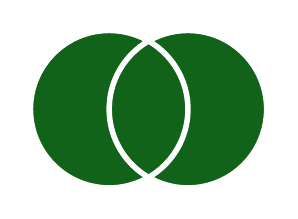
\begin{tikzpicture}[scale=1, color = white, line width = 2]
		\fill[aocfg1] (0,0) circle (1cm);
		\fill[aocfg1] (1,0) circle (1cm);
		\draw (0,0) circle (1cm); 
		\draw (1,0) circle (1cm);
	\end{tikzpicture}
    \end{center}
\end{textblock}

%%% A AND B
\begin{textblock}{5}(0,9)
	\MTitle{	
	\begin{tabular}{l} 
		A AND B \\
		A $\cap$ B
	\end{tabular}
	}
    \begin{center}
	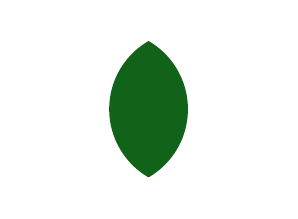
\begin{tikzpicture}[scale=1, color = white, line width = 2]
		\draw (1,0) circle (1);
		\draw[clip] (0,0) circle (1cm);
		\fill[aocfg1] (1,0) circle (1cm);
	\end{tikzpicture}
    \end{center}
\end{textblock}

%%% A NOT B
\begin{textblock}{5}(11,1)
    \MTitle{
	\begin{tabular}{l}
		A NOT B\\
		A $-$ B
	\end{tabular}
	}
    \begin{center}
	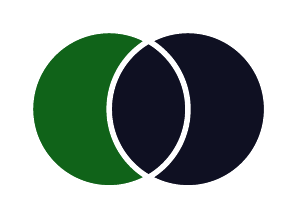
\begin{tikzpicture}[scale=1, color = white, line width = 2]
		\fill[aocfg1] (0,0) circle (1cm);
		\fill[aocbg] (1,0) circle (1cm);
		\draw (0,0) circle (1cm);
		\draw (1,0) circle (1cm);
	\end{tikzpicture}
    \end{center}
\end{textblock}

%%% A XOR B
\begin{textblock}{5}(11,9)
	\MTitle{	
	\begin{tabular}{l} 
		A XOR B \\
		\vphantom{A $\cap$ B}
	\end{tabular}
	}
    \begin{center}
	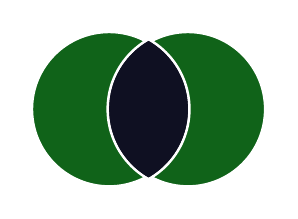
\begin{tikzpicture}[scale=1, color = white, line width = 2]
		\fill[aocfg1] (0,0) circle (1cm);
		\fill[aocfg1] (1,0) circle (1cm);
		\draw (1,0) circle (1);
		\draw[clip] (0,0) circle (1cm);
		\fill[aocbg] (1,0) circle (1cm);
		\fill[aocbg] (1,0) circle (1cm);
	\end{tikzpicture}
    \end{center}
\end{textblock}
\end{frame}


\end{document}
%%%
%%% TIME: 
%%% WORKING STATUS:
%%% COMMENTS:
